
%\documentclass[journal,onecolumn,12pt]{IEEEtran}
\documentclass[journal, 12pt, draftcls, onecolumn]{IEEEtran}
%\documentclass[a4paper, 10pt]{IEEEtran}
\hyphenation{op-tical net-works semi-conduc-tor}
\usepackage{graphicx}
\graphicspath{ {images/} }
\graphicspath{ {/home/zalperstein/Downloads/} }
\usepackage{cite}
\usepackage{setspace}
\usepackage{amsmath}
\usepackage{graphicx, subcaption}
\usepackage{subcaption}
\usepackage{float}
\floatstyle{plaintop}
\restylefloat{table}
\usepackage[justification=centering]{caption}
\usepackage{amssymb}
\usepackage{amsmath}
\usepackage{filecontents}
\usepackage{lipsum}
\usepackage{amsthm}
\usepackage{algorithmic,cite}
\usepackage{algorithm}
%\usepackage{cleveref}
\usepackage{authblk}
\usepackage{mathtools,xparse}
\usepackage{verbatim}

\DeclarePairedDelimiter{\norm}{\lVert}{\rVert}
\DeclarePairedDelimiter{\ceil}{\lceil}{\rceil}

\newtheorem {theorem} {Theorem}

%\singlespacing

\interdisplaylinepenalty=2500

%\def\BibTeX{{\rm B\kern-.05em{\sc i\kern-.025em b}\kern-.08em
%    T\kern-.1667em\lower.7ex\hbox{E}\kern-.125emX}}
\setcounter{page}{1}

\begin{document}
\title{Character Based Language Models Through Variational Sentence and Word Embeddings}
\author{Zaccary Alperstein and Kevin Bradley Dsouza}
%\affil{University of British Columbia, Vancouver, Canada}
%\\ email:\ kevin@ece.ubc.ca} 
%\IEEEoverridecommandlockouts
\IEEEpubid{\makebox[\columnwidth]{ 978-1-4799-2361-8/14/\$31.00~\copyright~2014 IEEE \hfill} \hspace{\columnsep}\makebox[\columnwidth]{ }} 

\maketitle
\thanks{}
\begin{abstract}
Language models have come of age recently with the introduction of Long-Short-Term-Memory based encoders, decoders and the advent of the attention mechanism. These models however work by generating one word at a time and cannot account for global sentence level context. In this project we propose a novel character based hierarchical variational autoencoder framework that can learn the word and sentence embeddings at the same time and can account for the global context. We couple this with an attention mechanism over the latent word embeddings to realize the end-to-end autoencoder framework.     
 
\end{abstract}

\section {Introduction} \label{intro}
Recurrent Neural Network language models (RNNLM) have shown superior results in unsupervised generative modelling for natural languages recently \cite{C1}. Supervised techniques like Machine Translation \cite{C2} and Image Captioning \cite{C3} have also achieved state of the art using these models. However, because RNNLM is an autoregressive probabilistic model that makes a series of step by step predictions, it does not model the global features such as topics, outside of its rich conditional distributions. This also means that the RNNLM will overfit to N-grams which appear frequently in the training data and thus stifles a diverse exploration of language.   

Variational autoencoder based language models have been developed recently to move from a hidden state deterministic representation of a sentence to a latent variable space. The bayesian latent variable model essential to the VAE allows for the encapsulation of latent variables into well defined sections of the neural network. It has been shown that these models are able to capture high level features, generate diverse sentences and also smoothly interpolate between sentences \cite{C4}. These models operate at the word level and thus find it difficult to handle languages with a high vocabulary and rich morphology like German, Russian and Turkish. They also cannot handle out of vocabulary words as they are built on a fixed predefined vocabulary.

The state of the art language models connect the encoder and the decoder through an attention mechanism. Attention mechanisms have become an indispensable part in sequence modelling because of their power to model dependencies without regard for the position in the input or the output sequence \cite{C2}, \cite{C5}. These are generally used in tandem with a reccurrent network, although, recently it has been shown that just an attention mechanism based architecture can achieve state of the art results at language modelling tasks \cite{C6}.   

In this project we aim to develop a character level language model to overcome the limitations of the word level models. We propose two hierarchical frameworks which differ in the way they incorporate the hierarchy, while both can jointly generate word and sentence level embeddings thus allowing us to form latent representations with sentence level context. We use a variational autoencoder to produce these latent representations and employ an attention mechanism over the latent word embeddings to account for long term dependencies in the sentence. The following sections elaborate on our proposal in depth. We present some existing literature in section \ref{litr}. Section \ref{framework} introduces the salient features of the two proposed frameworks. We discuss the evaluation methods and the datasets that will be used in section \ref{eval} and finally we end with the project timeline.   

\section{Literature Review}\label{litr} 
The Variational autoencoder (VAE) introduced in \cite{C7}, encodes the information to a latent variable space which can then be used to reconstruct the data using a decoder. Unlike traditional autoencoders \cite{C9}, the VAE drives the representation to a region instead of a single deterministic vector thus allowing for diversity in data generated from the vector space \cite{C4}, or even exhibit control over the generated text \cite{C8}. This nice property of variational autoencoders come from their principled bayesian semantics, where reconstruction is phrased as sampling from an approximate posterior distribution, with a strong regularization term that pushes the latent variables to a standard gaussian (shown below). Although variational Seq2Seq models are trickier to train, it is shown in \cite{C4} that it is possible to train a VAE to generate sentences from a continuous latent space. 

\[L_{ELBO}= E_{z \sim q(z|x)}[-log(p(x|z))] +  \int q(z|x)log(\dfrac{q(z|x)}{p(z)}) \]
Where $q(z|x)$ is the posterior distribution or encoder, $p(x|z)$ is the likelihood or decoder, and p(z) is a $N(0,I)$ gaussian in the non-hierarchical case.

Attention Mechanism helps us to weight over the input samples using an attention vector that is learned and thus can significantly improve performance of the Seq2Seq model \cite{C2}, \cite{C10}. Care has to be taken to incorporate attention over a variational space rather than a deterministic representation lest it overpower the model \cite{C11}.
Most of the traditional approaches employ a simple prior over the latent space like a normal distribution. This is convenient for training but converting the data distribution to a single mode can often lead to overly simplified representations which cannot faithfully reproduce the rich semantics of the data. Hierarchical VAEs are proposed in \cite{C12}, \cite{C13} to allow for greater modelling flexibility and structure.   

Word level language models cannot handle languages with a large vocabulary and rich morphology. In addition to that, when there is a large number of words in the dictionary, the parameters for the softmax itself dwarf the rest of those in the model for any given layer, as well as being a speed bottleneck in the network. Towards this end character level language models have been explored to mitigate this problem. A character level convolutional neural network coupled with a highway network and LSTM is used in \cite{C16}. It is shown that on languages with rich morphology (German, Spanish, Russian) the model outperforms the word level LSTM baselines at the same time using fewer parameters. Google's Neural Machine Translation System \cite{C15} addresses the issue of out of vocabulary words by dividing the words into a limited set of common sub word units called as "wordpieces" which handles translation of rare words and improves the overall accuracy of the system. They also go a step furthere, training hybrid models with characters for rare words. However it is not obvious that these characters actually allow them to translate out of vocabulary words, but is more for copying words like names between the input and output sentence. A hierarchical RNN architecture with multiple modules and different timescales is proposed \cite{C14}. A 30\% reduction in the number of parameters is seen with the use of these models with the accuracy in recognition staying the same. This model combines the word level feedback with the character level input to give robust predictions along with achieving significant memory reductions. 

Inspired by some of the above mentioned works we propose two novel hierarchical frameworks using variational autoencoders. Our frameworks are capable of producing the word and the sentence level representations jointly. We employ an attention mechanism over the variational word embeddings to account for the weighted importance of the input sequence and output one character at a time. A beam search will be carried out at the output to account for the varied sequential samples from the conditional distribution.  

\section {Framework} \label{framework}
Our desire of creating a hierarchical model with word embeddings, and global sentence representations may manifest in a variety of different ways for our variational autoencoder. Initially we explore an architecture which builds independent latent word representations, in the extreme case turning our model into a bag-of-words type encoder. With the fore-sight of potential local minima that our model may be trapped in, we then propose a second architecture which makes word embeddings dependent. Some potential novel applications of these models include:

1. Using them as an encoding step for a machine translation model

2. Exploration of varying sentence structures given a single context

\subsection{Framework 1: Hierarchy in the Sentence Based Latent representation}
This model builds independent word-based latent representations, saving the rich conditional hierarchy for encodings of the latent word representations in global sentence representations, which do encode positional dependence (Figure 1, without hierarchy). This allows us to make universal word representations for any arbitrary sequence of characters independent of context (at the extreme when the kl goes to 0 they are totally independent although this will likely not happen as it would harm reconstruction). This can be mostly taken care of by using a hierarchical prior (Figure 3).
In the simple case, we encode our characters into an RNN piece-by-piece until we hit an EOW (en of word) token, at which point we output the mean and variance of a posterior latent variable, and sample using the re-parametrization trick. This is repeated across the encoded sentence (Figure 1). We then average these random variables, which after a dense layer outputs a mean and variance as the hierarchical global latent representations. After this we can decode directly, or build a hierarchy with a deep attention mechanism (Figure 1). In the case that we build a hierarchy, our global latent variable is used as a query vector against the word-based latent variables, the output of which is pushed through a linear layer, or a dense then linear layer to parametrize the output distribution. This can be repeated n times where n is the depth of the hierarchy.In the decoder, we proceed from our global latent representation, and build a query by processing it with an RNN, which we use to reference the word embeddings with an attention mechanism (Figure 2). The output of this is then fed through the final RNN which outputs the probability of a character, given the latent representation. This is repeated until an EOS symbol is hit (Figure 2). The prior distribution can mimic the encoder, starting by sampling a standard gaussian for each of the desired words, averaging the samples, and then following the rest of the encoder to parametrize the other latent variables (i.e. dense, then sample like in Figure 1). Indeed the generative model here will likely not work very well, as is usual for unigram models. However the posterior still has useful application. To make a more rich generative model, we can make our prior fully dependent (Figure 3).
\begin{figure}
\centering
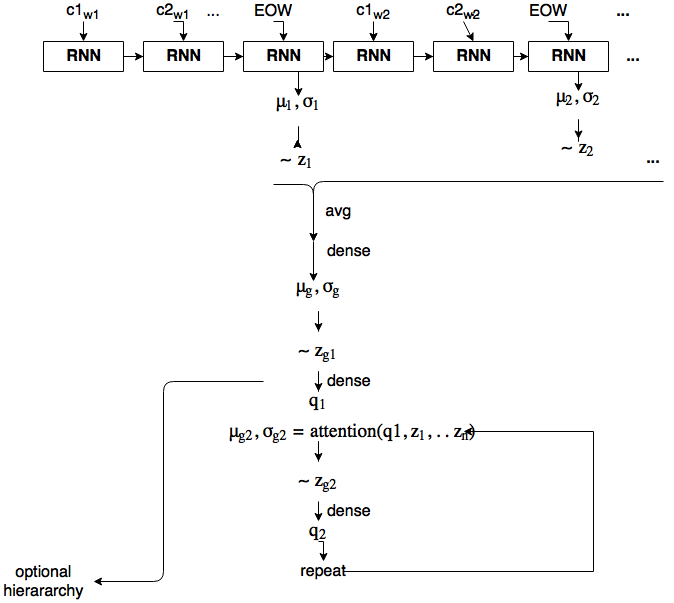
\includegraphics[scale=0.5]{fig1_charvae.png}
\caption{Uncorrelated word embeddings, with hierarchy in the sentence latent representation only. Here 'Zg' is a hierarchical random variable which includes correlation with the latent word embeddings.}
\end{figure}

\begin{figure}
\centering
\includegraphics[scale=0.5]{fig2b_charVAE.png}
\caption{Decoder.}
\end{figure}

\begin{figure}
\centering
\includegraphics[scale=0.5]{fig1B_charVAE.png}
\caption{Correlated prior distribution.}
\end{figure}

A potential problem with the aforementioned model is that VAEs tend to be very conservative with their use of latent variables, and so it might be easier for the VAE to shut off all latent variables associated with the words and instead pack everything into the single final output vector. This problem is especially amplified in the case of a standard gaussian word-based representation. To avoid this we propose to incentivize the VAE with a fully hierarchical word-based latent representation.

\subsection{Framework 2: Hierarchy in the RNN}
Here our model is quite similar to the one mentioned above, with the key difference being that our encoding RNN builds latent representations conditioned of the previous latent variable sampled. To do this we propose to run the RNN across each character, after the first EOW we output a mean and variance as before. However this time we reset the hidden state of the RNN, and only pass in the latent variable as a representations of the previous parts of the sentence. In this case our last hidden variable is highly correlated with the previous random variables, serving not only as a word embedding, but a word embedding which is highly context specific. Due to the immense depth of this stochastic network as is, our initial experiments will not include adding a deeper hierarchy like in the previous section, however it is optional and so it is depicted in Figure 4. The decoding in this case is done exactly like the previous architecture (Figure 2), and the prior used in this case is the same as that which was already mentioned to solve the problem of independent word representations (Figure 3).

\begin{figure}
\centering
\includegraphics[scale=0.5]{fig2_charVAE.png}
\caption{Hierarchical approximate posterior, or encoder with a correlated hierarchy in the RNN. Optionally more correlation may be employed to make a deep hierarchical sentence representation 'Zg'}
\end{figure}


\section {Evaluation} \label{eval}
For evaluation we can use importance-weighted log-likelihood \cite{C17} estimates in order to directly compare with previously published language models directly. With these more accurate log-likelihood estimates we can make a fair comparison with perplexity as well.
\[LL \sim E_{h_1,h_2,...,h_k \sim q(h|x)}[log \dfrac{1}{k} \sum_{i=1}^k \dfrac{p(x,h_i)}{q(h_i|x)}]\]
and the perplexity measure:
\[2^{H(p)}= 2^{-\sum_x p(x) log_2 p(x)}=2^{average(\sum_x^N NLL_{estimate(x)})}\]

Furthermore we can compare BLEU scores to gauge the quality of the generated sentences from the generative distribution. Finally, we can examine the outputs qualitatively (as is frequently done with generative models), as well as homotopies, and the ability of our model to sample coherent sentences given a context.

We test our framework on English Penn TreeBank (PTB) dataset \cite{C18}, utilizing the standard training (0-20), validation (21-22), and test (23-24) splits. Also, once this is done, we aim to test with some of the other morphologically rich languages like Czech, German, French, Spanish, Russian, and Arabic \cite{C19}, \cite{C20}. 

\section{Timeline} \label{timeline}
\begin{enumerate}
    \item Week 1: Implement framework 2 - \emph{Hierarchy in the RNN.} Algorithm writing and debugging. 
    \begin{itemize}
        \item Kevin - Encoder 
        \item Zac - Decoder / structuring objective function
    \end{itemize}
    \item Week 2,3: 
    \begin{itemize}
        \item Zac - Hyper parameter tuning and optimization.
        \item Kevin - Evaluation on PennTreeBank 
    \end{itemize}
    \item Week 4: Zac, Kevin - Evaluation on other languages and experimenting with the aforementioned framework 1 - \emph{Hierarchy in the Sentence Based latent representation}, if time permits.  
\end{enumerate}


\begin{thebibliography}{20}
\bibitem{C1}
Tom ́aˇs Mikolov, Stefan Kombrink, Luk ́aˇs Burget, Jan Honza Cˇernocky`, and Sanjeev Khudanpur. 2011. Extensions of recurrent neural network language model. In Proc. ICASSP.
\bibitem{C2}
Dzmitry Bahdanau, Kyunghyun Cho, and Yoshua Bengio. 2015. Neural machine translation by jointly learning to align and translate. In Proc. ICLR.
\bibitem{C3}
Oriol Vinyals, Alexander Toshev, Samy Bengio, and Dumitru Erhan. 2015. Show and tell: A neural image caption generator. In Proc. CVPR.
\bibitem{C4}
Bowman, S. R.; Vilnis, L.; Vinyals, O.; Dai, A. M.; Jozefowicz, R.; and Bengio, S. 2016. Generating sentences from a continuous space. CoNLL.
\bibitem{C5}
Yoon Kim, Carl Denton, Luong Hoang, and Alexander M. Rush. Structured attention networks. In International Conference on Learning Representations, 2017.
\bibitem{C6}
A. Vaswani, N. Shazeer, N. Parmar, J. Uszkoreit, L. Jones, A. N. Gomez, L. Kaiser, and I. Polosukhin, “Attention is all you need,” arXiv preprint arXiv:1706.03762, 2017
\bibitem{C7}
Diederik P Kingma and Max Welling. 2013. Auto- encoding variational Bayes. arXiv preprint arXiv:1312.6114.
\bibitem{C8}
Zhiting Hu, Zichao Yang, Xiaodan Liang, Ruslan Salakhutdinov, and Eric P. Xing. 2017. Toward con- trolled generation of text. In Proceedings of the 34th International Conference on Machine Learning. vol- ume 70, pages 1587–1596.
\bibitem{C9}
Geoffrey E Hinton and Ruslan R Salakhutdinov. 2006. Reducing the dimensionality of data with neural net- works. Science 313(5786):504–507.
\bibitem{C10}
Alexander M. Rush, Sumit Chopra, and Jason We- ston. 2015. A neural attention model for ab- stractive sentence summarization. In Proceed- ings of the 2015 Conference on Empirical Methods in Natural Language Processing. pages 379–389. https://doi.org/10.18653/v1/D15-1044.
\bibitem{C11}
Bahuleyan, Hareesh, et al. "Variational Attention for Sequence-to-Sequence Models." arXiv preprint arXiv: 1712.08207 (2017).
\bibitem{C12}
Sønderby, Casper Kaae, et al. "Ladder variational autoencoders." Advances in neural information processing systems. 2016.
\bibitem{C13}
Goyal, Prasoon, et al. "Nonparametric variational auto-encoders for hierarchical representation learning." arXiv preprint arXiv:1703.07027 (2017).
\bibitem{C14}
Hwang, Kyuyeon, and Wonyong Sung. "Character-level language modeling with hierarchical recurrent neural networks." Acoustics, Speech and Signal Processing (ICASSP), 2017 IEEE International Conference on. IEEE,
2017.
\bibitem{C15}
Wu, Yonghui, et al. "Google's neural machine translation system: Bridging the gap between human and machine translation." arXiv preprint arXiv:1609.08144 (2016).
\bibitem{C16}
Kim, Yoon, et al. "Character-Aware Neural Language Models." AAAI. 2016.
\bibitem{C17}
Burda, Grosse, et al. "Importance Weighted Autoencoders." arxiv. 2016.
\bibitem{C18}
Marcus, M.; Santorini, B.; and Marcinkiewicz, M. 1993. Building a Large Annotated Corpus of English: the Penn Treebank. Compu- tational Linguistics 19:331–330.
\bibitem{C19}
Available online: http://www.statmt.org/wmt13/translation-task.html
\bibitem{C20}
Available online: http://opus.nlpl.eu/News-Commentary.php
\end{thebibliography}



\ifCLASSOPTIONcaptionsoff
  \newpage
\fi


\bibliographystyle{IEEEtran}

\end{document}


